\def\year{2017}\relax
%File: formatting\mathrm{-}instruction.tex
\documentclass[letterpaper]{article}
\usepackage{aaai17}
\usepackage{amsmath}
\usepackage{amsthm}
\usepackage{times}
\usepackage{helvet}
\usepackage{courier}
\usepackage{graphicx}
\usepackage{subfigure}
\usepackage{mdwmath}
\usepackage{mdwtab}
\usepackage{amssymb}
\usepackage{booktabs}
\usepackage{algorithm}
\usepackage{pifont}
\usepackage[noend]{algpseudocode}
\usepackage{balance}
\usepackage{bm}
\usepackage{ulem}
\usepackage{array}
\usepackage{balance}
\usepackage{multirow}
\usepackage{multicol}
\frenchspacing
\setlength{\pdfpagewidth}{8.5in}
\setlength{\pdfpageheight}{11in}
\usepackage[marginal]{footmisc}
%\pdfinfo{
%/Title (Appendices)
%}
\setcounter{secnumdepth}{0}  
 \begin{document}
% The file aaai.sty is the style file for AAAI Press 
% proceedings, working notes, and technical reports.
%
%\title{Appendices}
%\author{
%}
%\maketitle





\newtheorem{Theorem}{\bf{Theorem}}
\newtheorem{Assumption}{\bf{Assumption}}
\newtheorem{Lemma}{\bf{Lemma}}
\newtheorem{Corollary}{\bf{Corollary}}

\section{Symbol notations}
\label{sect_notations}
The symbols used in the paper and their notations are presented in Figure \ref{symbol_notations}. 
\begin{figure}
\centering
\subfigure{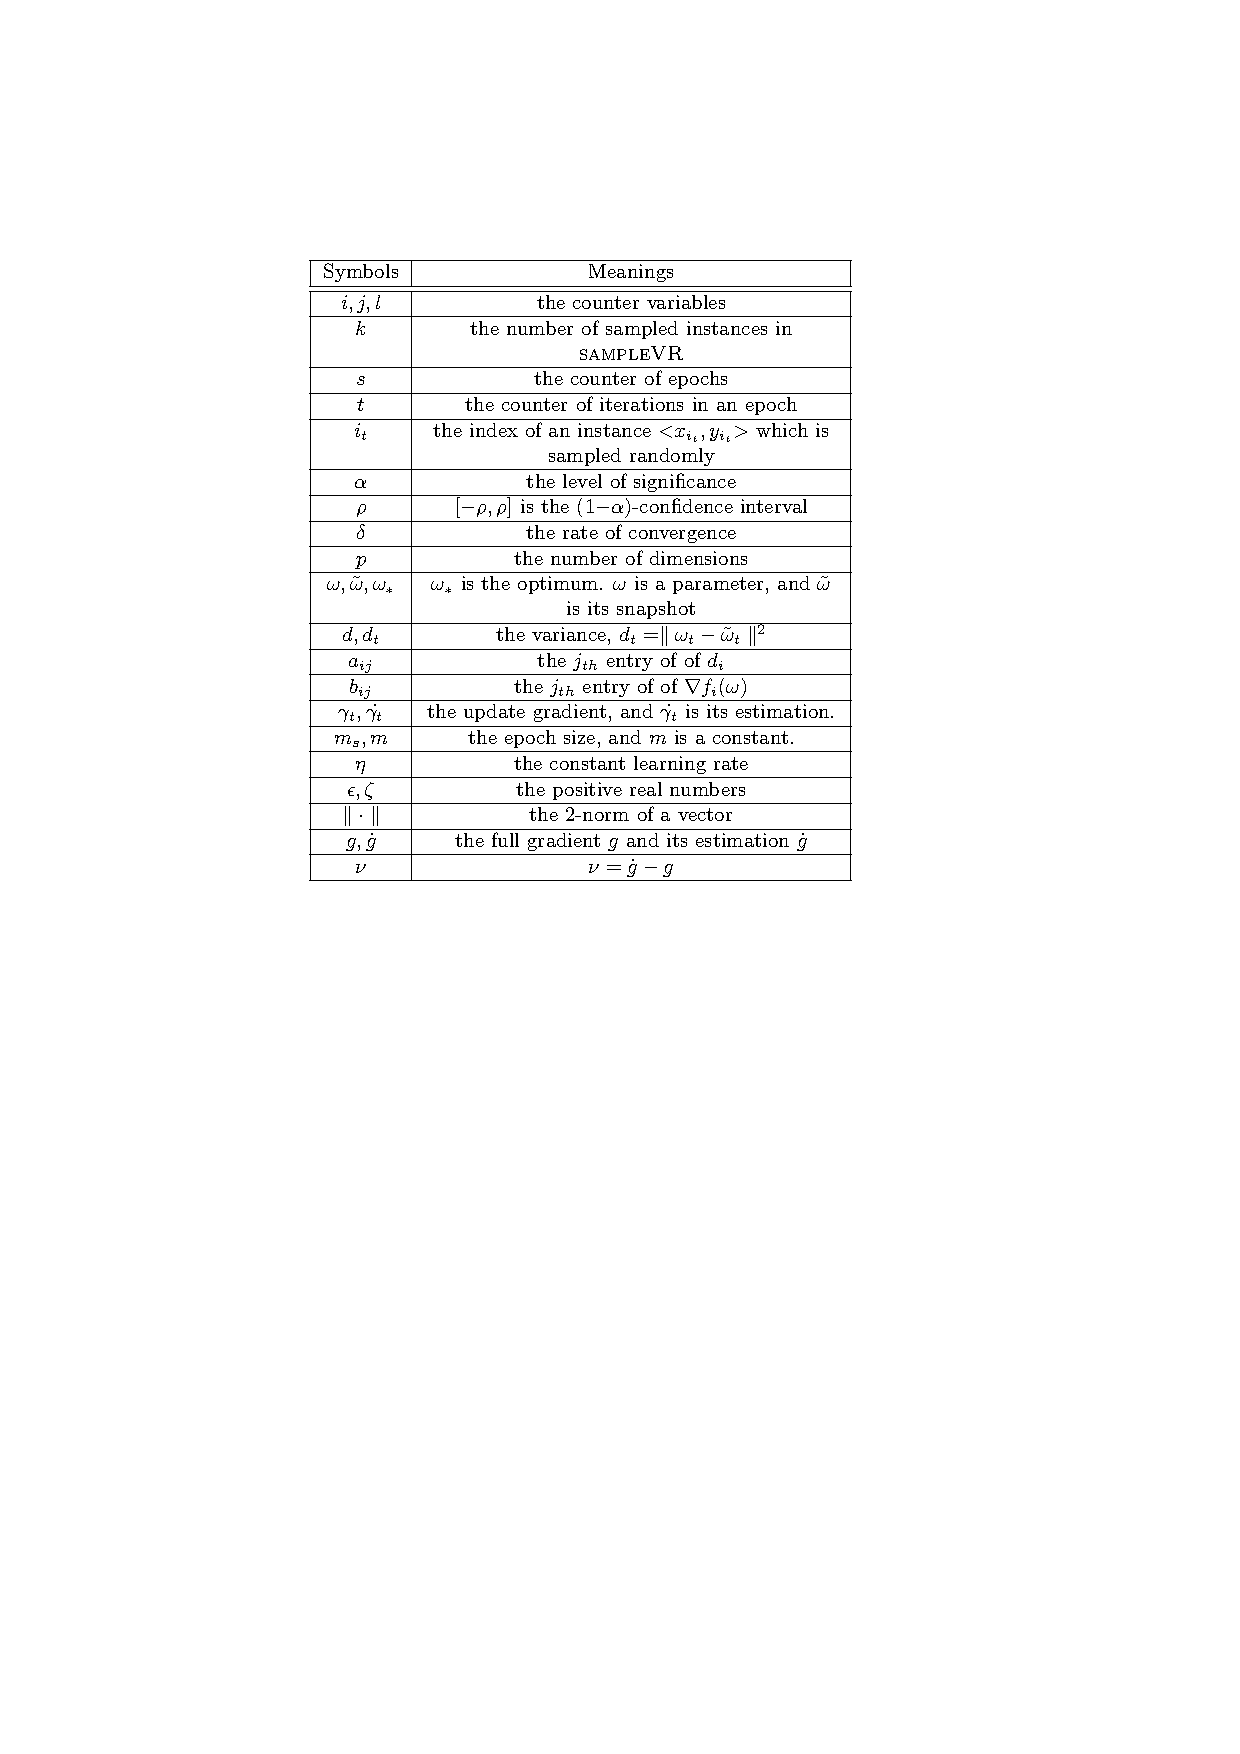
\includegraphics[width=1\columnwidth]{symbol_notations}}
\caption{Symbols used in the paper and their notations.}
\label{symbol_notations}
\end{figure}





\section{Proofs}
\label{sect_proofs}
In order to make the proofs of the theorems in this paper easy to read, the  assumptions are re-presented here. 

%The optimisation objective is:
%\begin{equation}
%\label{equa_loss_minimization}
%\min F(\omega),~~~~~F(\omega)=\frac{1}{n}\sum\limits_{i=1}^n f_i(\omega)+R(\omega)\\
%\end{equation}. The assumptions are shown as follows:


\begin{Assumption}
Each a function $f_{i_t}$ with $i_t\in\{1,2, ..., n\}$ in Equ. 1 is $L$-Liptchiz continuous, that is, for any two parameters $\omega_i$ and $\omega_j$:
\label{assumption_liptchiz}
\begin{equation}
\label{equa_l_smooth} 
f_{i_t}(\omega_i)\le f_{i_t}(\omega_j)\mathrm{+}\nabla f_{i_t}(\omega_j)^\mathrm{T} (\omega_i\mathrm{-}\omega_j)\mathrm{+}\frac{L}{2}\parallel \omega_i\mathrm{-}\omega_j\parallel^2
 \end{equation}.

\end{Assumption}

\begin{Assumption}
\label{assumption_strongly_convex}
The function $F$ in Equ. 1 is $\mu$-strongly convex, that is, for any two parameters $\omega_i$ and $\omega_j$:
\begin{equation}
F(\omega_i)\ge F(\omega_j)\mathrm{+}\nabla F(\omega_j)^\mathrm{T} (\omega_i\mathrm{-}\omega_j)\mathrm{+}\frac{\mu}{2}\parallel \omega_i\mathrm{-}\omega_j\parallel^2
\end{equation}.

\end{Assumption}

After that, all the proofs of the theorems presented in the main document are illustrated as follows:

\begin{Theorem}
\label{theorem_vr_lower_bound}
   After $t$ iterations in an epoch, the distance $d_t$ holds that $d_t \mathrm{=} \eta^2 \sum\limits_{j=1}^p\left(  \sum\limits_{i=1}^t a_{ij}  \right)^2$. Furthermore, $d_t$ has an upper bound such that 
   $d_t \mathrm{\le} \eta^2 t^2p  \left( \frac{1}{tp}\sum\limits_{i=1}^t   \sum\limits_{j=1}^p   a_{ij}^2 \right)$, and a lower bound such that $d_t  \mathrm{\ge} \eta^2t^2p \left(\frac{1}{tp}\sum\limits_{i=1}^t   \sum\limits_{j=1}^p   a_{ij}\right)^2$.
\end{Theorem}
\begin{proof}
\begin{equation}
\begin{array}{ll}
d_{t} = \parallel \omega_{t}\mathrm{-}\tilde{\omega} \parallel^2 
=\parallel \omega_{{t\mathrm{-}1}}\mathrm{-}\eta \gamma_{t-1} \mathrm{-}\tilde{\omega} \parallel^2\\
= \parallel \omega_{0}\mathrm{-}\tilde{\omega}  \mathrm{-} \sum\limits_{i=1}^t \eta \gamma_i \parallel^2 
=\parallel \mathrm{-}\sum\limits_{i=1}^t \eta \gamma_i \parallel^2\\
= \eta^2 \sum\limits_{j=1}^p\left(  \sum\limits_{i=1}^t a_{ij}  \right)^2
\end{array}
\end{equation}. Taking the expectation of $i_{i_t}$,  $\mathbb{E}(\gamma_t) = \mathbb{E}(\nabla f_{i_t}(\omega_t)-\nabla f_{i_t}(\tilde{\omega})+\nabla F(\tilde{\omega})) = \nabla F(\omega_{t})$ holds,   and we thus obtain the upper bound of the distance:
\begin{equation}
\begin{array}{ll}
d_{t} = \eta^2 t^2 \sum\limits_{j=1}^p\left( \frac{1}{t} \sum\limits_{i=1}^t a_{ij}  \right)^2
\le \eta^2 t^2 \sum\limits_{j=1}^p\left( \frac{1}{t} \sum\limits_{i=1}^t a_{ij}^2  \right)\\
= \eta^2 t  \left( \sum\limits_{i=1}^t   \sum\limits_{j=1}^p   a_{ij}^2 \right) 
= \eta^2 t^2p  \left( \frac{1}{tp}\sum\limits_{i=1}^t   \sum\limits_{j=1}^p   a_{ij}^2 \right)
\end{array}
\end{equation}, and the lower bound of the distance:
\begin{equation}
\begin{array}{ll}
d_{t} = \eta^2 p \left( \frac{1}{p} \sum\limits_{j=1}^p\left( \sum\limits_{i=1}^t a_{ij}  \right)^2\right)
\ge \eta^2 p \left(  \frac{1}{p}  \sum\limits_{j=1}^p \sum\limits_{i=1}^t a_{ij}  \right)^2\\
= \frac{\eta^2}{p} \left(\sum\limits_{i=1}^t   \sum\limits_{j=1}^p   a_{ij}\right)^2  
= \eta^2t^2p \left(\frac{1}{tp}\sum\limits_{i=1}^t   \sum\limits_{j=1}^p   a_{ij}\right)^2
\end{array}
\end{equation}.
\end{proof}


\begin{Lemma}
\label{lemma_nu}
Given $\nu = \frac{1}{k}\sum\limits_{t=1}^k  \nabla f_{i_t}(\omega) - \frac{1}{n}\sum\limits_{i=1}^n \nabla f_i(\omega)$, we obtain
$\mathbb{E}_{i_t}\parallel \nu  \parallel^2 \le \frac{4L(n-k)}{nk}\left(F(\omega) - F(\omega_\ast)\right)$ holds for any an arbitrary parameter $\omega$.
\end{Lemma}
\begin{proof}
Given any two arbitrary parameters $\omega_i$ and $\omega_j$,  $f_{i_t}(\omega_i)\le f_{i_t}(\omega_j)\mathrm{+}\nabla f_{i_t}(\omega_j)^\mathrm{T} (\omega_i\mathrm{-}\omega_j)\mathrm{+}\frac{L}{2}\parallel \omega_i\mathrm{-}\omega_j\parallel^2$ holds according to Assumption  \ref{assumption_liptchiz}. Let $\omega_i = \omega  - \frac{1}{L}\nabla f(\omega)$, and $\omega_j = \omega$, and then we obtain
\begin{equation}
\begin{array}{ll}
f_{i_t}(\omega_i) \le f_{i_t}(\omega)-\frac{1}{2L}\parallel  \nabla f_{i_t}(\omega)   \parallel^2
\end{array} 
\end{equation}.  $i_{t}$ is taken on the expectation, and we thus obtain
\begin{equation}
\begin{array}{ll}
\mathbb{E}_{i_t}\left(\parallel  \nabla f_{i_t}(\omega)   \parallel^2 \right) \le 2L \mathbb{E}_{i_t}\left( f_{i_t}(\omega) - f_{i_t}(\omega_i) \right)   \\
\le 2L (F(\omega) - F(\omega_i) )  \le 2L (F(\omega) - F(\omega_\ast))
\end{array} 
\end{equation}. Here, $\omega_\ast$ is the optimum of the loss function.   Without loss of generality, suppose that indices of the sampled $k$ instances are $i_t\in\{1,2, ..., k\}$.
\begin{equation}
\begin{array}{ll}
\mathbb{E}_{i_t}\parallel \nu  \parallel^2 
= \mathbb{E}_{i_t}\left( \parallel \frac{1}{k}\sum\limits_{i=1}^k  \nabla f_{i}(\omega) \mathrm{-} \frac{1}{n}\sum\limits_{i=1}^n \nabla f_i(\omega) \parallel^2  \right)    \\
= \frac{1}{(nk)^2}  \mathbb{E}_{i_t}\parallel  (n-k)\sum\limits_{t=1}^k \nabla f_{i}(\omega)-k \sum\limits_{i=k+1}^n \nabla f_{i}(\omega) \parallel^2      \\
\le  \frac{2(n-k)^2}{(nk)^2}  \sum\limits_{i=1}^k \mathbb{E}_{i_t} \parallel  \nabla f_{i}(\omega) \parallel^2  + \frac{2k^2}{(nk)^2}  \sum\limits_{i=k+1}^{n} \mathbb{E}_{i_t} \parallel  \nabla f_{i}(\omega) \parallel^2    \\
\le \frac{4L(n-k)}{nk}(F(\omega) - F(\omega_\ast))
\end{array} 
\end{equation}. 
\end{proof}
\begin{Theorem}
\label{Theorem_converge}
If $\delta=\frac{\mu m \eta^2 (8Ln-8Lk+4Lnk)+nk}{  \mu m nk \eta (1-2\eta L)  } < 1$ with $\sqrt{\frac{1}{2\mu m (4Ln-4Lk+3Lnk)}} < \eta < \frac{1}{4(4Ln-4Lk+3Lnk)}\sqrt{\frac{nk(2\mu mnk - 32Ln+ 32 Lk -24 Lnk)}{\mu m}}$ holds, \textsc{sampleVR} makes the training loss converge as
$F(\tilde{\omega}_{s\mathrm{+}1}) \mathrm{-} F(\omega_\ast)  \le \delta [F(\tilde{\omega}_s)\mathrm{-}F(\omega_\ast)]$.
\end{Theorem}
\begin{proof}
Construct an auxiliary function $h_i(\omega)=f_i(\omega)\mathrm{-}f_i(\omega_\ast)\mathrm{-}\nabla f_i(\omega_\ast)^\mathrm{T}(\omega\mathrm{-}\omega_\ast)$, and $h_i(\omega_\ast)=\min\limits_\omega h_i(\omega)$ holds because of $\nabla h_i(\omega_\ast)=0$. Thus, $h_i(\omega_\ast)\le \min\limits_\eta [h_i(\omega\mathrm{-}\eta \nabla h_i(\omega))]$ holds. According to Assumption \ref{assumption_liptchiz}, we obtain
$h_i(\omega_\ast)\le\min\limits_\eta [h_i(\omega)\mathrm{-}\eta \parallel \nabla h_i(\omega) \parallel^2\mathrm{+}\frac{1}{2} L \eta^2 \parallel  \nabla h_i(\omega)  \parallel^2  ] 
=h_i(\omega)\mathrm{-}\frac{1}{2L}\parallel  \nabla h_i(\omega) \parallel^2$.  That is, 
$\parallel   \nabla f_i(\omega)  \mathrm{-} \nabla f_i(\omega_\ast)   \parallel^2 \le 2L [ f_i(\omega)  \mathrm{-}  f_i(\omega_\ast)  \mathrm{-}\nabla f_i(\omega_\ast)^{\mathrm{T}}(\omega\mathrm{-}\omega_\ast)  ]$. By summing this inequality over $i=\{1,2, ..., n\}$, and using the fact that $\nabla F(\omega_\ast)=0$, we obtain $
\frac{1}{n} \sum\limits_{i=1}^n \parallel  \nabla f_i(\omega)  \mathrm{-} \nabla f_i(\omega_\ast)  \parallel^2  \mathrm{\le}   2L [F(\omega)\mathrm{-}F(\omega_\ast)] $. $i_t$ is a random variable which is sampled from $\{1,2, ...,n\}$ randomly. Taking the expectation of $i_t$, we obtain 
\begin{equation}\label{equa_1}
\begin{array}{ll}
\mathbb{E}_{i_t}(\parallel  \nabla f_{i_{t}}(\omega) \mathrm{-} \nabla f_{i_{t}}(\omega_{\ast}) \parallel^2) \\
= \frac{1}{n} \sum\limits_{i=1}^n \parallel  \nabla f_i(\omega)  \mathrm{-} \nabla f_i(\omega_\ast)  \parallel^2 \\
\le 2L [F(\omega)\mathrm{-}F(\omega_\ast)] 
\end{array} 
\end{equation}.  
\begin{equation}\label{equa_2}
\begin{array}{ll}
\mathbb{E}_{i_t}\parallel  \dot{\gamma}_{t} \parallel^2  
= \mathbb{E}_{i_t} \parallel \nabla f_{i_{t}}(\omega_{t}) \mathrm{-} \nabla f_{i_{t}}(\tilde{\omega}_s)  \mathrm{+} \nabla F(\tilde{\omega}_s) \mathrm{+} \nu \parallel^2\\
\le 2\mathbb{E}_{i_t} \parallel \nabla f_{i_{t}}(\omega_{t}) \mathrm{-} \nabla f_{i_{t}}(\omega_{\ast}) \parallel^2 \mathrm{+}\\
 2 \mathbb{E}_{i_t} \parallel  \nabla f_{i_{t}}(\tilde{\omega}_{s}) \mathrm{-} \nabla f_{i_{t}}(\omega_{\ast}) \mathrm{-} \nabla F(\tilde{\omega}_s)   \mathrm{-} \nu  \parallel^2  \\
\le 2\mathbb{E}_{i_t} \parallel \nabla f_{i_{t}}(\omega_{t}) \mathrm{-} \nabla f_{i_{t}}(\omega_{\ast}) \parallel^2  \mathrm{+} \\
4 \mathbb{E}_{i_t} \parallel  \nabla f_{i_{t}}(\tilde{\omega}_{s}) \mathrm{-} \nabla f_{i_{t}}(\omega_{\ast}) \mathrm{-} \nabla F(\tilde{\omega}_s) \parallel^2 \mathrm{+} 4\mathbb{E}_{i_t} \parallel \nu  \parallel^2 \\ 
\le 2\mathbb{E}_{i_t} \parallel \nabla f_{i_{t}}(\omega_{t}) \mathrm{-} \nabla f_{i_{t}}(\omega_{\ast}) \parallel^2  \mathrm{+} 4 \mathbb{E}_{i_t} \parallel  \nabla f_{i_{t}}(\tilde{\omega}_{s}) \mathrm{-} \nabla f_{i_{t}}(\omega_{\ast}) \\
\mathrm{-} \mathbb{E}_{i_t} \left ( \nabla f_{i_t}(\tilde{\omega}_s) \mathrm{-} \nabla f_{i_t}(\omega_\ast)   \right)\parallel^2   \mathrm{+} \frac{16L(n-k)}{nk} ( F(\tilde{\omega}_s) - F(\omega_\ast))    \\ 
\le 2\mathbb{E}_{i_t} \parallel \nabla f_{i_{t}}(\omega_{t}) \mathrm{-} \nabla f_{i_{t}}(\omega_{\ast}) \parallel^2  \mathrm{+} \\
4 \mathbb{E}_{i_t} \parallel  \nabla f_{i_{t}}(\tilde{\omega}_{s}) \mathrm{-} \nabla f_{i_{t}}(\omega_{\ast}) \parallel^2 \mathrm{+} \frac{16L(n-k)}{nk} ( F(\tilde{\omega}_s) - F(\omega_\ast))\\
\le 4L [F(\omega_t)\mathrm{-}F(\omega_\ast)] \mathrm{+} \left( 8L+ \frac{16L(n-k)}{nk}\right) [F(\tilde{\omega}_s)\mathrm{-}F(\omega_\ast)]
\end{array} 
\end{equation}.  The third inequality uses Lemma \ref{lemma_nu},  the fourth inequality uses $\mathbb{E}[\xi\mathrm{-}\mathbb{E}\xi]^2 \le \mathbb{E}\xi^2$, and the fifth inequality uses (\ref{equa_1}). Therefore, we obtain 
\begin{equation}
\begin{array}{ll}
\mathbb{E}_{i_t}\parallel  \omega_{t+1}\mathrm{-}\omega_\ast \parallel^2\\
=\parallel  \omega_{t}\mathrm{-}\omega_\ast  \parallel^2  \mathrm{-}2\eta(\omega_t\mathrm{-}\omega_\ast)^\mathrm{T}\mathbb{E}_{i_t}\dot{\gamma}_{t}  \mathrm{+}  \eta^2 \mathbb{E}_{i_t}\parallel  \dot{\gamma}_{t}  \parallel^2  \\
\le \parallel  \omega_{t}\mathrm{-}\omega_\ast  \parallel^2  \mathrm{-}2\eta(\omega_t\mathrm{-}\omega_\ast)^\mathrm{T}\nabla F(\omega_t) \mathrm{+} \\
\eta^2 \left(  4L [F(\omega_t)\mathrm{-}F(\omega_\ast)] \mathrm{+} \left( 8L+ \frac{16L(n-k)}{nk}\right) [F(\tilde{\omega}_s)\mathrm{-}F(\omega_\ast)] \right)  \\ 
\le \parallel  \omega_{t}\mathrm{-}\omega_\ast  \parallel^2  \mathrm{-}2\eta( F(\omega_t) \mathrm{-} F(\omega_\ast) ) \mathrm{+} \\
\eta^2 \left(  4L [F(\omega_t)\mathrm{-}F(\omega_\ast)] \mathrm{+} \left( 8L+ \frac{16L(n-k)}{nk}\right) [F(\tilde{\omega}_s)\mathrm{-}F(\omega_\ast)]\right)  \\ 
= \parallel  \omega_{t}\mathrm{-}\omega_\ast  \parallel^2  \mathrm{-}2\eta(1\mathrm{-}2\eta L) [F(\omega_t) \mathrm{-} F(\omega_\ast) ] \mathrm{+} \\
\frac{16L(n-k)+8Lnk}{nk} \eta^2 [F(\tilde{\omega}_s)\mathrm{-}F(\omega_\ast)]
\end{array} 
\end{equation}. The first inequality uses (\ref{equa_2}), and the second inequality holds because that $F(\omega)$ is convex.  We thus obtain 
\begin{equation}
\begin{array}{ll}
\parallel  \omega_{m}\mathrm{-}\omega_\ast \parallel^2\\
= \parallel  \omega_{0}\mathrm{-}\omega_\ast  \parallel^2  \mathrm{-}2\eta(1\mathrm{-}2\eta L)\sum\limits_{t=0}^{m-1} [F(\omega_t) \mathrm{-} F(\omega_\ast) ] \mathrm{+} \\
\frac{16L(n-k)+8Lnk}{nk} m \eta^2 [F(\tilde{\omega}_s)\mathrm{-}F(\omega_\ast)]\\
=\parallel  \tilde{\omega}_{s}\mathrm{-}\omega_\ast  \parallel^2  \mathrm{-}2\eta(1\mathrm{-}2\eta L)m \left(\frac{1}{m}\sum\limits_{t=0}^{m-1} [F(\omega_t) \mathrm{-} F(\omega_\ast) ] \right)\mathrm{+} \\
\frac{16L(n-k)+8Lnk}{nk} m \eta^2 [F(\tilde{\omega}_s)\mathrm{-}F(\omega_\ast)]\\
%\le \parallel  \tilde{\omega}_{s}\mathrm{-}\omega_\ast  \parallel^2  \mathrm{-}2\eta(1\mathrm{-}2\eta L)m [F(\frac{1}{m}\sum\limits_{t=0}^{m-1} \omega_t) \mathrm{-} F(\omega_\ast) ] \mathrm{+} \\
%\frac{16L(n-k)+8Lnk}{nk} m \eta^2 [F(\tilde{\omega}_s)\mathrm{-}F(\omega_\ast)]\\
= \parallel  \tilde{\omega}_{s}\mathrm{-}\omega_\ast  \parallel^2  \mathrm{-}2\eta(1\mathrm{-}2\eta L)m \mathbb{E}_t[F(\tilde{\omega}_{s+1}) \mathrm{-} F(\omega_\ast) ] \mathrm{+} \\
\frac{16L(n-k)+8Lnk}{nk} m \eta^2 \mathbb{E}_t [F(\tilde{\omega}_s)\mathrm{-}F(\omega_\ast)]
\end{array} 
\end{equation}. The second equality  holds because of $\omega_0=\tilde{\omega}_s$. The third equality holds when we take expectation of $t$. The reason is that $\tilde{\omega}_{s+1}$  is identified by picking $\omega_t$ with $t\in\{0,1, ..., m-1\}$ randomly, and $\tilde{\omega}_s$ is a constant in an epoch.  Thus, 
\begin{equation}
\begin{array}{ll}
2\eta(1\mathrm{-}2\eta L)m \mathbb{E}_t [F(\tilde{\omega}_{s\mathrm{+}1}) \mathrm{-} F(\omega_\ast) ] \\
\le  \parallel  \tilde{\omega}_{s}\mathrm{-}\omega_\ast  \parallel^2 \mathrm{+} \frac{16L(n-k)+8Lnk}{nk} m \eta^2 \mathbb{E}_t[F(\tilde{\omega}_s)\mathrm{-}F(\omega_\ast)] \\ 
\le \frac{2}{\mu}\mathbb{E}_t[ F(\tilde{\omega}_{s}) \mathrm{-}  F(\omega_\ast)  ]\\
 \mathrm{+} \frac{16L(n-k)+8Lnk}{nk} m \eta^2 \mathbb{E}_t[F(\tilde{\omega}_s)\mathrm{-}F(\omega_\ast)]
\end{array} 
\end{equation}. The second inequality holds due to the Assumption \ref{assumption_strongly_convex}. Therefore, we obtain $\delta=\frac{\mu m \eta^2 (8Ln-8Lk+4Lnk)+nk}{  \mu m nk \eta (1-2\eta L)  } < 1$ with $\sqrt{\frac{1}{2\mu m (4Ln-4Lk+3Lnk)}} < \eta < \frac{1}{4(4Ln-4Lk+3Lnk)}\sqrt{\frac{nk(2\mu mnk - 32Ln+ 32 Lk -24 Lnk)}{\mu m}}$, and thus the training loss converges such that
$\mathbb{E}_t[F(\tilde{\omega}_{s\mathrm{+}1}) \mathrm{-} F(\omega_\ast)]  \le \delta \mathbb{E}_t[F(\tilde{\omega}_s)\mathrm{-}F(\omega_\ast)]$.  Thus, the Theorem \ref{Theorem_converge} have been proved.
\end{proof}



%-------------------------------------------------------------------------------------------------------------------------------------------------------------------------------------------------%
%The first inequality uses $\mathbb{E}_{i_t}\dot{\gamma}_t = \nabla F(\omega_t)$, and the second inequality uses the convex property of the loss function.  Summing the above inequality over $t=\{0,1, ..., m\mathrm{-}1\}$, we obtain
%\begin{equation}
%\begin{array}{ll}
%\mathbb{E}_{i_t}\parallel  \omega_{m}\mathrm{-}\omega_\ast \parallel^2  \\
%\le \parallel  \omega_{0}\mathrm{-}\omega_\ast  \parallel^2  \mathrm{-}2\eta(1\mathrm{-}2\eta L) \sum\limits_{i=0}^{m\mathrm{-}1} [F(\omega_i) \mathrm{-} F(\omega_\ast) ]  \\
%\mathrm{+} \frac{16L(n-k)+8Lnk}{nk} \eta^2 m [F(\tilde{\omega}_s)\mathrm{-}F(\omega_\ast)]\\ 
%\end{array} 
%\end{equation}. When $\tilde{\omega}_{s\mathrm{+}1}$ is randomly identified from the sequence   $\{ \omega_0, ...,  \omega_{m_{s}\mathrm{-}1}   \}$. Taking expectation on $t$, we obtain $\tilde{\omega}_{s\mathrm{+}1}  = \mathbb{E} (\omega_t)$ with $t=\{0,1, ..., m-1   \}$. Therefore, 
%\begin{equation}
%\begin{array}{ll}
%\mathbb{E}_{t}\parallel  \omega_{m}\mathrm{-}\omega_\ast \parallel^2  \mathrm{+} 2\eta(1\mathrm{-}2\eta L) m [F(\tilde{\omega}_{s\mathrm{+}1}) \mathrm{-} F(\omega_\ast) ] \\
%\le \mathbb{E}\parallel  \omega_{0}\mathrm{-}\omega_\ast  \parallel^2 \mathrm{+} \frac{16L(n-k)+8Lnk}{nk} \eta^2 m [F(\tilde{\omega}_s)\mathrm{-}F(\omega_\ast)] \\ 
%= \parallel  \tilde{\omega}_{s\mathrm{+}1}\mathrm{-}\omega_\ast  \parallel^2 \mathrm{+} \frac{16L(n-k)+8Lnk}{nk} \eta^2 m [F(\tilde{\omega}_s)\mathrm{-}F(\omega_\ast)] \\ 
%\le \frac{2}{\mu}\parallel  F(\tilde{\omega}_{s\mathrm{+}1}) \mathrm{-}  F(\omega_\ast)  \parallel^2 \mathrm{+} \frac{16L(n-k)+8Lnk}{nk} \eta^2 m [F(\tilde{\omega}_s)\mathrm{-}F(\omega_\ast)]
%\end{array} 
%\end{equation}. The second equality holds because of $\omega_{s+1}  = \mathbb{E}( \omega_t )$ with $t=\{0,1, ..., m-1\}$. The third inequality holds due to the Assumption \ref{equa_gamma_convex}.
%Thus, 
%\begin{equation}
%\begin{array}{ll}
%\left ( \eta(1\mathrm{-}2\eta L) m  \mathrm{-}  \frac{1}{\mu}   \right  ) [F(\tilde{\omega}_{s\mathrm{+}1}) \mathrm{-} F(\omega_\ast) ] \\
%\le 8 L \eta^2 m [F(\tilde{\omega}_s)\mathrm{-}F(\omega_\ast)]
%\end{array} 
%\end{equation}.
%-------------------------------------------------------------------------------------------------------------------------------------------------------------------------------------------------%





\begin{Theorem}
\label{theorem_gradient_complexity}
\textsc{sampleVR} requires at least  $\frac{\ln \zeta}{\ln \delta}m\mathrm{+}\left( \mathrm{-} \frac{\log\frac{\alpha}{2}}{2\epsilon} (\frac{\ln \zeta}{\ln \delta}+1)(\frac{\ln \zeta}{\ln \delta})\right)$ atomic gradient calculations with $\delta=\frac{\mu m \eta^2 (8Ln-8Lk+4Lnk)+nk}{  \mu m nk \eta (1-2\eta L)  }$ to achieve $\mathbb{E}_t[F(\tilde{\omega}_s)\mathrm{-}F(\omega_\ast)] \le \zeta \mathbb{E}_t[F(\omega_0)\mathrm{-}F(\omega_\ast)]$.
\end{Theorem}
\begin{proof}

The required atomic gradient calculations for the $s_{th}$ epoch is denoted by $G_\mathrm{s}$. We obtain
$G_s = k \mathrm{+}m = \mathrm{-} \frac{s\log\frac{\alpha}{2}}{\epsilon}\mathrm{+}m$.
If $\mathbb{E}_t[F(\tilde{\omega}_s)\mathrm{-}F(\omega_\ast)] \le \zeta \mathbb{E}_t[F(\omega_0)\mathrm{-}F(\omega_\ast)]$ holds, then we obtain $\delta^s = \zeta$ according to Theorem \ref{Theorem_converge}, that is, $s=\frac{\ln \zeta}{\ln \delta}$. Therefore, the total  gradient complexity is 
$\frac{\ln \zeta}{\ln \delta}m\mathrm{+}\left( \mathrm{-} \frac{\log\frac{\alpha}{2}}{2\epsilon} (\frac{\ln \zeta}{\ln \delta}+1)(\frac{\ln \zeta}{\ln \delta})\right)$ atomic gradient calculations with $\delta=\frac{\mu m \eta^2 (8Ln-8Lk+4Lnk)+nk}{  \mu m nk \eta (1-2\eta L)  }$. 


\end{proof}








\end{document}
